\clearpage

\def\chaptertitle{Dynamic Range Thresholding on Streams}

\lhead{\emph{\chaptertitle}}

\chapter{\chaptertitle}
\label{ch:drts}

For certain applications, one may be motivated to define a more general type of RTS query, in which the interval of interest \textit{evolves over time} with the data stream. Consider our first motivating example of a trader wanting to be alerted the moment some volume $\tau$ of Apple shares is traded between some price levels $[200, 205]$. In practice, the price levels of interest is likely to evolve over the day of the trading, or even widen with volatility. For example, a trader may wish to register a query of the form: \textit{notify me when $\tau$ volume of Apple shares are traded within 10\% of Apple's volume-weighted average price}. As one may recall, the volume-weighted average price (vwap) formula is given by 
$$\text{vwap} = \frac{\sum_{e} v(e) \cdot w(e)}{\sum_{e}w(e)}$$
which we clearly see evolves over the evolution of the data stream $\{e_i\}_{i=1}$, meaning that the endpoints of the traders interval of interest also evolves over time.

In this chapter, we formally define this more general type of query, which we call a \textit{dynamic range threshold query} (DRTS query), then demonstrate that with minor adjustments, the DT algorithm discussed in \cref{ch:rts} is able to solve this more general type of query, though only when the number of \textit{distinct} DRTS queries is small (we will formally define exactly what we mean by \textit{distinct} later on). Finally, we introduce a novel approximation algorithm to handle a large number of distinct DRTS queries. 


\section{Problem Definition}
\label{sec:drts-problem-definition}

We define a Dynamic RTS (DRTS) query and then the dynamic range thresholding on streams problem.

\begin{definition}[Dynamic RTS query] A Dynamic RTS query is defined by a time-index triple $(R_t, \tau, f)$ where $\tau\in\mathbb{Z}$ is a \textit{threshold}, $f$ is a monotonically increasing  endpoint function and $R_t\subseteq \mathbb{R}^d$ is a time-indexed subset of the data space formed by axis-parallel rectangles. For $t =1,2,\dots$ the end points of each axis parallel rectangle $[a_t, b_t]$ are updated according to $[a_{t+1}, b_{t+1}]_i = [f(a_t), f(b_t)]_i$ for $i=1,\dots,d$ and $t=1,2,\dots$
\end{definition}

The dynamic range thresholding on streams problem is defined exactly as in \cref{sec:rts-definition}, though now with DRTS queries. That is, if a given query is issued after receiving $e_j$ for some $j\geq 1$ then for $t\geq j+1$ we define $S(q,t)$ to represent the elements $e_{j+1},e_{j+2},\dots,e_t$ that \textit{stab} $R_q$. That is, 
$$S(q, t) := \{e_i | j < i \leq t \text{ and } e_i \in R_q\}$$
Define
$$W(q, t) := \sum_{e\in S(q,t)}w(e)$$
Then the \textit{maturity time} of a query $q$ is the smallest $t$ such that $W(q,t)\geq \tau_q$. Our goal is to simultaneously support a set of $m$ DRTS queries and to correctly report the maturity time of a each query as well as the operations Register$(q)$: accept a new query at the current moment (after the arrival of $e_n$) and Terminate$(q)$: stop a given query $q$.

Some useful examples of DRTS queries are the following

\begin{example}[\textit{Equal Step DRTS}] Consider $m$ DRTS queries $(R_{qt}, \tau_q, f)$ on the one-dimensional data space  $\mathbb{R}$ with common endpoint function $f(x) = x + \Delta$ for a fixed constant $\Delta\in\mathbb{R}$. Conceptually, such an endpoint function moves the each query to the left or right (depending on the sign of $\Delta$) by a factor of $\Delta$ after each time step.
\end{example}

\begin{example}[\textit{Equal Expansion DRTS}] Consider $m$ DRTS queries $(R_{qt}, \tau_q, f)$ on the one-dimensional data space  $\mathbb{R}$ with common endpoint function $f(x) = \Delta x$  for a fixed constant $\Delta\in\mathbb{R}$. Conceptually, such an endpoint function expands the length of each query by an order of $\Delta$ on each time step.
\end{example}
    
We note that definition 4.1 leaves few restrictions on the possible choices for the endpoint function $f$, only that it be monotonically increasing so that the interval remains well defined after each time step. One could therefore supply a multivariate function $f(x,t)$ such as $f(x, t) = x + \Delta_t$ for some sequence $\{\Delta_t: t\geq1\}$. Thus, proposed solutions to the DTS problem must be able to solve these types of queries also. 

\section{Benchmark Solutions}
\label{sec:drts-benchmark-solutions}

The introduction of endpoint functions limits the feasibility of the many of the benchmark solutions previously explored in \cref{sec:benchmark-solutions}. The reason being, many of these Data Structures are created on the intervals. In the DRTS context, all $m$ query intervals could possibly change significantly at each time stamp, forcing a complete rebuild of the Data Structure.

One benchmark solution which is robust enough to manage changes to the intervals that are present in the case of the DRTS problem is following naive algorithm:

\begin{algorithm}
\caption{Naive RTS}\label{alg:naive-drts}
\begin{algorithmic}[1]
\Procedure{Naive-DRTS}{query set $Q^*$}
\State \text{for each $q\in Q^*$ initialise $c_q\gets 0$}
\For{ \text{each stream element $e_t$}}
\For{ \text{each $q\in Q^*$}}
\State \text{calculate $R_t$ using endpoint function $f$}
\State \text{if $e\in R_t$ set $c_q \gets c_q + w(e)$}
\State \text{if $c_q \geq \tau_q$, mature query $q$}
\EndFor
\EndFor
\EndProcedure
\end{algorithmic}
\end{algorithm}

\section{DT Algorithm For DRTS Queries}
\label{sec:drts-dt-algorithm}

The goal of this section is to demonstrate that with minor enhancements, the DT algorithm can solve certain DRTS queries. Moreover, we then characterise exactly what DRTS queries our new algorithm is able to solve. First we need to consider two versions of the Dynamic Range Thresholding on Streams problem: 

\begin{definition}[Distinct \& Non-Distinct Dynamic RTS]
    Conisder $m$ DRTS queries $(R_{t}^q, \tau_q, f_q)$ if all queries share the same endpoint function, that is for all $1\leq i\leq  j\leq m$ we have $f_i = f_j$ then we say this is an instance of the \textit{Non-Distinct} DRTS problem. In the case where any of the two queries have different endpoint functions, we call this an instance of the \textit{Distinct DRTS} problem.
\end{definition}

Clearly, the non-distinct DRTS problem offers us a simpler problem instance from which we can first design our enhanced algorithm. We then apply some standard techniques to extend to the distinct case. 

\subsection{Non-Distinct DRTS}
\label{ssec:non-distinct-rts}

We consider the scenario in which all queries are registered with the same end point function and to illuminate the discussion, we suppose our queries are an instance of the \textit{Equal-Step} case (see Example 4.1). 

Given it's effectiveness in the standard RTS problem We would like to continue using the DT algorithm from \cref{sec:DT-algorithm}. One initial thought may be to insert new intervals or create new endpoint trees for each timestamp $t$, as the intervals of the registered queries change according to $f$. Simple analysis will show that this adds an unavoidable $O(m\log m)$ factor to the element processing cost, inflating the runtime of the algorithm back to the quadratic $O(nm\log^2 m)$. Instead, our approach will focus on pre-processing the stream value $v(e_t)$ at each time step. 

The crucial observation is that in the non-distinct DRTS problem, we can map the problem to an instance of the standard RTS problem with the following \textit{shifting lemma}. 

\begin{lemma}[Shifting Lemma]
    let $(R_n, \tau, f)$ be an RTS query such that $f$ is invertable and $e_n$ be the $n^{th}$ stream element. Let $R_0$ denote the value of the query's interval at the time it was registered. Then 
    $$v(e_n) \in R_n \iff f^{-1}_{(n)}(v(e_n))\in R_0$$
    where $f^{-1}_{(n)} = \underbrace{f^{-1}\cdots f^{-1}}_{n \text{ times}}(v(e_n))$
\end{lemma}

To describe our algorithms, we will also use the following definitions

\begin{definition}[Shifting, Shift]
    For a given query $(R, \tau, f)$ registered at time $n$ and a stream element $e_{n^\prime}$ with $n^\prime > n$ we refer to the operation $v(e_{n^\prime})\gets f^{-1}_{(n^\prime - n)}(v(e_{n^\prime}))$ as \textit{shifting $v(e_{n^\prime})$} or simply as performing a \textit{shift}
\end{definition}

Sticking with our example of the \textit{Equal-Step DRTS}, suppose that the endpoint function of each query is $f(x) = x+\Delta$. So for a given query registered with interval $R_0 = [a,b]$, after $n$ time steps the interval becomes $R_n = [a + \Delta n, b+\Delta_n]$. By the shifting lemma, we have $v(e_n) \in R_n \iff v(e_n) - \Delta n \in [a,b]$ which we notice is a stabbing query on the in initial interval $R_0$ - suggesting that we can include the shifting lemma as a pre-processing step to element processing, and then run the original DT-algorithm.

The astute reader may now ask what happens for queries registered at different time steps. Consider one interval $R_0 = [a, b]$ registered at time $n$ and another interval $R^\prime_0 = [c,d]$ registered at time $n^\prime \neq n$. Suddenly it becomes unclear whether we should apply the shift $v(e_n) - \Delta n$ or $v(e_n) - \Delta n^\prime$. Fortunately, the logarithmic rebuilding technique we use to enable the register procedure for new queries provides us a means of handling this.

Recall from \cref{sec:logarithmic-rebuilding} and \cref{ssec:unconstrained-DT-algorithm} when a new query is inserted, we find the smallest $i = 1,\dots,h=\log m$ such that $\mathcal{T}_i$ is empty. We then destroy all trees $\mathcal{T}_1,\dots,\mathcal{T}_{i-1}$, and combine their queries, along with the newly registered query into $\mathcal{T}_i$. In the context of the DRTS problem, this presents an opportunity \textit{update} each query in the newly formed $\mathcal{T}_i$ such that they all require the same shift. To illustrate this, suppose that the query sets on trees $\mathcal{T}_1,\dots,\mathcal{T}_{i-1}$ require shifts $f^{-1}_{(n_1)},\dots,f^{-1}_{(n_{j-1})}$. When the queries are grouped together to construct $\mathcal{T}_{j}$, first update the endpoints of the registered query to $f_{(n_1)}, \dots, f_{(n_{j-1})}$. This allows us to effectively consider all queries in $\mathcal{T}_j$ being registered simultaneously, and thus require the same shift. We formalise this with the following procedure for performing a register

\begin{algorithm}\label{alg:DT+-register}
\begin{algorithmic}[1]
\Procedure{DRTS::Register}{$q$}
\State \text{Determine smallest $i$ such that $\mathcal{T}_i = \emptyset$}
\EndProcedure
\end{algorithmic}
\end{algorithm}

Necessary to show the correctness of our algorithm, we formalise and prove the following lemma.

\begin{lemma}
    
\end{lemma}
\begin{proof}
    We show the claim with a simple induction argument on $n$, the number of Register operations performed. The base case occurs at the commencement of the algorithm, when all queries are initially registered and placed into a singular tree.
\end{proof}

By incorporating the two techniques of first applying the shifting lemma, and then updating the endpoints of queries when performing register operations, we arrive at the DT+ Algorithm. 

\begin{algorithm}
\caption{DT+ Algorothm}\label{alg:DT+-algorithm}
\begin{algorithmic}[1]
\Require $Q^* \gets m$ \text{ RTS queries $(R_q, \tau_q)$}
\State \text{Build end point tree $\mathcal{T}$ from endpoints in $Q^*$}
\For{ $q \in Q^*$}
    \State \text{Find canonical node set $U_q$}
    \State \text{Create instance of \cref{alg:dist-tracking} on $U_q$}
\EndFor
\State \text{Commence data stream} 
\For{$e_t$ for $t = 1,2,\dots$}
    \For{\text{endpoint tree $\mathcal{T}_1,\dots,\mathcal{T}_{\log m}$}}
    \State \text{Shift $v(e_t)$ based on $\mathcal{T}_i$}
    \State \text{Trace $e_t$ through $\mathcal{T}$ based on Jurisdiction Interval}
    \State \text{Update node counters $c(v) \gets c(v)+1$ for each $v\in V(\mathcal{T})$ traced}
    \State \text{Perform \cref{alg:slack-inspection} for each $v\in V(\mathcal{T})$ traced}
    \EndFor
\EndFor
\end{algorithmic}
\end{algorithm}

\cref{alg:DT+-algorithm} and the provides an illuminating characterisation of when we can extend the DT algorithm to solve the DRTS problem, namely, we need to be able to perform the shifting operation and be able to do so quickly. We close our discussion with the following theorem:

\begin{theorem}[Correctness \& Runtime]
    Consider $m$ DRTS queries with equal endpoint function $f$. If $f$ is invertable and $f^{-1}$ can be computed in $O(1)$ time then \cref{alg:DT+-algorithm} correctly solves the Non-distinct DRTS problem in $O(n\log^{d+1}m + m\log^{d+1}m\log\tau_{\max})$
\end{theorem}
\begin{proof}
    Correctness follows from the shifting lemma and Lemma 4.5. reducing the problem to an instance of Range Thresholding on Streams, which is solved by \cref{alg:DT+-algorithm}. The only difference between \cref{alg:DT+-algorithm} and the original DT algorithm is the inclusion of step 9, which by assumption can be performed in $O(1)$. 
\end{proof}

\newpage
\subsection{Distinct DRTS}
\label{ssec:distinc-DRTS}
We now turn our attention to more general distinct DRTS problem, in which the endpoint function may differ between registered query. Clearly, we can no longer apply the shifting technique when dealing with an endpoint tree containing queries with different endpoint functions. Instead, we need to consider how to best \textit{group} or \textit{bucket} the queries such that we can run instances of \cref{alg:DT+-algorithm} on the resulting group.

The most straightforward approach is to simply bucket the queries based on their end point function. That is, divide the query set into disjoint subsets $S_1,\dots, S_k$ such each query in $S_i$ shares the same endpoint function $f$. Then create an instance of \cref{alg:DT+-algorithm} on $S_1,\dots,S_k$. Each incoming stream element is then passed through each instance. That is

\begin{algorithm}
\caption{DRTS-Bucketing I}\label{alg:DRTS-bucketing}
\begin{algorithmic}[1]
\Require $Q^* \gets m$ \text{ RTS queries $(R_q, \tau_q, f_q)$}
\State \text{Form query set $Q_1,\dots,Q_k$ based on $f_q$}
\State \text{$DT(Q_i) \gets $ instance of \cref{alg:DT+-algorithm} on $Q_i$ for $i=1,\dots,k$}
\For{$e_t$ for $t=1,2,\dots$}
    \State \text{Process $e_t$ on $DT(Q_i)$ for $i=1,\dots,k$} 
\EndFor
\end{algorithmic}
\end{algorithm}

Recalling that our goal is to avoid a quadratic $O(nm)$ runtime, we now ask how many different endpoint functions can \cref{alg:DRTS-bucketing} allow before falling into the quadratic trap?  

 As before let $Q$ be a set of equal-step queries, though now $Q$ is comprised of queries with $k$ different shift factors; $\Delta_1, \dots, \Delta_k$. As before, we can partition $Q$ into queries of equal shift factor, which we write as $Q_{\Delta_1}, \dots, Q_{\Delta_k}$. As $Q_{\Delta_i}$ are disjoint we have 
$\sum_{i=1}^{k} |Q_{\Delta_i}| = |Q| = m$. As above, we build DT instances on each of the partitions of $Q$. To process an incoming data element, we pass the element through the endpoint tree of $Q_{\Delta_1},\dots, Q_{\Delta_k}$. The total runtime of our algorithm on a stream of $n$ elements is therefore

\begin{align*}
\sum_{i=1}^{k}\text{run-time}(Q_{\Delta_i}) &= \sum_{i=1}^{k} n\log |Q_{\Delta_i}| + |Q_{\Delta_i}|\log^2 |Q_{\Delta_i}| \log\tau_{max} \\
&= \sum_{i=1}^{k} n\log |Q_{\Delta_i}| + \sum_{i=1}^{k}  |Q_{\Delta_i}|\log^2 |Q_{\Delta_i}| \log\tau_{max} 
\end{align*}
Recall the first summation corresponds to the element processing cost, and the latter summation corresponds to the communication cost of each distributed tracking instance. Let's examine the first term
\begin{align*}
    \sum_{i=1}^{k} n\log |Q_{\Delta_i}| &= n\sum_{i=1}^{k}\log |Q_{\Delta_i}| \\
    &= n \log \left(\prod_{i=1}^{k}|Q_{\Delta_i}| \right)
\end{align*}
We can bound the product using the arithmetic mean-geometric mean inequality which states that: 
$\sqrt[n]{\prod_{i=1}^{n} s_i} \leq \frac{1}{n}\sum_{i=1}^{n}s_i$. Applying to the above we have
\begin{align*}
     n \log \left(\prod_{i=1}^{k}|Q_{\Delta_i}| \right) &\leq n \log\left(
     \frac{1}{k}\sum_{i=1}^{k}|Q_{\Delta_i}|\right)^k \\
     &= n\log^k (m/k) \\ 
     &= nk\log (m/k)
\end{align*}
The second summation is a little more trickier to tightly analyse, but we make some simple upper bounds. First, the $\log\tau_{max}$ term in the summation technically corresponds to the maximum threshold among each $Q_{\Delta_{i}}$ set, though clearly each of these will be less than or equaly to the global maximum threshold over all $Q_{\Delta_i}$, so we let $\tau_{max}$ denote this global threshold. Secondly, let $|Q_{\Delta}^*| = \max_{1\leq i \leq k} |Q_{|\Delta_i}|\leq m$ it now follows that 
\begin{align*}
    \sum_{i=1}^{k}  |Q_{\Delta_i}|\log^2 |Q_{\Delta_i}| \log\tau_{max} &\leq \sum_{i=1}^{k}  |Q_{\Delta_i}|\log^2 |Q_{\Delta}^*| \log\tau_{max} \\
    &= m\log^2 |Q_{\Delta}^*| \log\tau_{max} \\
    &\leq m\log^2 m \log\tau_{max}
\end{align*}
Which is the same in terms of big-$O$ as before. This makes sense, as splitting up and processing an element over each of the $k$ DT instances may increase the element processing cost, but it would not alter the total messaging cost of the algorithm. This brings the total runtime analysis to: 
$$O(nk\log (m/k) + m\log^2 m \log\tau_{max})$$
which the worst case deprecates to $O(nm)$ runtime when we have as many distinct endpoint functions as we do queries. It is now clear that so long as $k = O(\log m)$ we can preserve a runtime of $\Tilde{O}(n+m)$. We conclude the analysis of this section with the following theorem. 

\begin{theorem}[Correctness and Time Complexity]
    For a collection of $m$ DRTS queries with $k$ distinct endpoint functions, and a stream of length $n$, \cref{alg:DRTS-bucketing} correctly solves the DRTS problem in runtime $O(nk\log(m/k) + m\log^2 m\log\tau_{\max})$. In the case that $k = O(\log m)$ the runtime is polylogarithmic.
\end{theorem}



\newpage
\section{$\varepsilon$ - Fuzzy DRTS}

Theorem 4.7 suggests that designing an \textit{exact} DRTS algorithm is difficult for problem instances with a large number of distinct endpoint functions. We now ask, can we bucket our queries in such a way that we trade some accuracy for speed? In this following section, we formalise an approximated version of the DRTS problem, and propose (as far as we know) an entirely novel approach to grouping DRTS queries to solve the problem.

\subsection{Problem Definition}

An $\varepsilon$-fuzzy variant can be formulated for both the RTS and DRTS problems.  Recall that an RTS query $(R, \tau)$ consists of a threshold $\tau \in\mathbb{R}$ and an interval $R \subseteq\mathbb{R}$. For a data stream $e_1,e_2,\dots$ where each stream element contains a value $v(e_t)\in\mathbb{R}$ and weight $w(e_t)\in\mathbb{Z}$ the goal is to report the exact moment that $\sum_{e\in S} w(e) \geq \tau$ where $S$ is the set of stream elements $e$ such that $v(e)\in R$. 

For a given RTS query $(R, \tau)$ we can define the $\varepsilon$-\textit{fuzzy} version of the query as follows. Let $R = [l, r]$ the original interval, and define the \textit{$\varepsilon$ core interval} as $\text{core}(R) := [l+\varepsilon/2, r-\varepsilon/2]$. In the case that $R\subseteq\mathbb{R}^d$, the core interval is defined analogously on each axis $1,\dots,d$.  

If the query is issued after receiving $e_j$ for some $j\geq 1$ then for $t\geq j+1$ we define $S(q,t)$ to represent the elements $e_{j+1},e_{j+2},\dots,e_t$ that \textit{stab} core($R$). That is, 
$$S(q, t) := \{e_i | j < i \leq t \text{ and } e_i \in \text{core}(R)\}$$
Analogously define $S^\prime$ to be the set of stream elements $e_{j+1},e_{j+2},\dots$ that stab the interval in general
$$S^\prime(q, t) := \{e_i | j < i \leq t \text{ and } e_i \in R\}$$
Define
$$W(q, t) := \sum_{e\in S(q,t)}w(e) \quad \text{ and } \quad W^\prime(q, t) := \sum_{e\in S^\prime(q,t)}w(e)$$
The goal of the the $\varepsilon$-fuzzy Range Threshold on Streams problem is to report the first moment that $\tau\geq W(q,t)$ or $\tau \geq W^\prime(q,t)$.

That is, in the $\varepsilon$-fuzzy variant, we record all stream elements that stab $\text{core}(R)$, but may also possible record elements that stab the outer core of the interval as well. We  extend the definition of $\varepsilon$-fuzzy intervals above to define an $\varepsilon$-fuzzy dynamic RTS query analogously. 

\subsection{Novel Bucketing Algorithm}
\label{sec:novel-bucketing-algorithm}
We now propose our algorithm for the $\varepsilon$-fuzzy DRTS problem. The intuition behind our algorithm is that we can now bucket queries that don't share the exact same endpoint function, but they are \textit{approximately} close for long enough time so that the core region of each interval remains \textit{covered}. Over the course of our algorithm, we provide simple corrective measures to ensure our this approximated cover is well maintained. 

We describe our algorithm below in psuedocode before proving its runtime and correctness. 


Input: a collection of $m$ DRTS queries of the form $(R_i, \tau_i, \Delta_i)$ and core threshold $\varepsilon$

\begin{enumerate}
    \item For each query set the approximated shift factor $\Delta_i^\prime \leftarrow \lceil\Delta_i\rceil_2$

    \item Form groups of queries $Q_1, \dots, Q_k$ such that any queries $i,j\in Q$, $\Delta_i^\prime = \Delta_j^\prime$. Denote by $\Delta^\prime_{Q_i}$ the common approximation shift factor for the group.

    \item For each group of queries, set 
    \begin{align*}
        & t^{(1)}_{Q} \leftarrow \min_{i\in Q} \lfloor\varepsilon/2(\Delta_i^\prime - \Delta_i) \rfloor \\
        & t^{(2)}_{Q} \leftarrow \min_{i\in Q} \lfloor-\varepsilon/2(\Delta_i/2^\prime - \Delta_i)\rfloor
    \end{align*}

    \item For each query set $Q_i$, instantiate an instance of the DT+ Algorithm on the the elements of $Q_i$, with shifting factor $\Delta^\prime_{Q_i}$

    \item Commence the data stream for $t=1,2,\dots$. For each Query set $Q_1,\dots,Q_k$ every $t_Q^{(1)}$ time stamps set $\Delta_Q^\prime \leftarrow \Delta_Q^\prime / 2$, then every $t_Q^{(2)}$ time stamps set $\Delta_Q^\prime \leftarrow \Delta_Q^\prime \times 2$. Repeat this altenating throughout the life of the algorithm. \\
    \\
    Once $\Delta^\prime_{Q_1}, \dots, \Delta^\prime_{Q_k}$ have been checked and possibly updated, process the incoming stream element through instance of the DT+ algorithm on $Q_1, \dots, Q_k$, reporting query maturation through the DT+ algorithm.
\end{enumerate}

We now demonstrate the correctness of our algorithm, and formally prove that it escapes the quadratic trap with a polylogarithmic $\Tilde{O}(n+m)$ runtime. 

\begin{lemma}[Correctness ]For each query $(R_i, \tau_i, \Delta_i)$ The algorithm correctly maintains a count of all stream elements that stab the $\varepsilon$-core of $R_i$
    
\end{lemma}

\begin{proof}
    For a given query $(R_i, \tau_i, \Delta_i)$, let $l(t), r(t)$ be the left and right endpoints of the original interval at time $t$. Let  $l^\prime(t), r^\prime(t)$ be the the left and right endpoints of the approximated interval maintained by the algorithm at time $t$. \\
    \\
    We note that in order for the core interval to be maintained, it must always lay within the approximated interval $[l^\prime(t), r^\prime(t)]$. We now show that this is always the case. \\
    \\
    For each query, the initial approximation factor $\Delta_i$ is approximated by $\Delta_i^\prime = \lceil \Delta_i\rceil_2 \geq \Delta_i$. As the approximated interval is moving rightward \textit{faster}, there must be a time at which $l^\prime(t)$ will extend beyond the left endpoint of the core interval $l(t) + \varepsilon/2$. To identify when this occurs we find 
    \begin{align*}
        l^\prime(t) &= l(0) + \Delta_i^\prime t > l(0) + \varepsilon/2 + \Delta_i t \\
        &\implies (\Delta_i^\prime - \Delta_i) t > \varepsilon/2 \\
        & \implies t > \frac{\varepsilon}{2(\Delta_i^\prime - \Delta_i)} \quad\quad (1)
    \end{align*}
    Similarly, throughout the running of our algorithm, the approximation factor changes to $\Delta_i^\prime = \lfloor \Delta_i \rfloor_2 \leq \Delta_i$, in which case the approximated interval moves \textit{slower} than the original interval.By noting that the core interval is maintained by the approximated interval so long as $r^\prime(t)\geq r(t) - \varepsilon/2$. By similar argument to above we find that this is violated when 
    $$ t > \frac{-\varepsilon}{2(\Delta_i^\prime - \Delta_i)}  \quad\quad (2)$$
    We note that $(1)$ and $(2)$ are calculated by steps 3 of the algorithm. Moreover, the updating of $\Delta_Q^\prime$ in step 5 of the algorithm ensures that no condition is violated
\end{proof}

\textbf{Lemma} (Time Complexity). \textit{For a set of $m$ queries $(R_i, \tau_i, \Delta_i)$  
 and a data stream of length $n$, the Algorithm runs in $O(nk\log (m/k) + m\log^2 m \log\tau_{\text{max}})$ where $k = O(\log \Delta_{\text{max}})$} 
 \begin{proof}
    Steps 1 through to 4 of the algorithm can be viewed as \textit{preprocessing}, all of which can be readily seen to require $\Theta(m)$ time. The bulk of the run time can be attributed to step 5; which requires that we check and update each approximation factor $\Delta^\prime_{Q_i}$, and then process the stream element on each of the DT+ instances running on $Q_1,\dots, Q_k$. \\
    \\
    Firstly, as each $Q_1,\dots, Q_k$ is formed by the approximation factors $\lceil \Delta_i\rceil_2$, we have $k\leq \log_2\Delta_{\text{max}}$ where $\Delta_{\text{max}}$ is the largest $\Delta_i$ in our query set. Step 5 of the algorithm therefore requires a loop over the $O(\log\Delta_{\text{max}})$ groups to check violation conditions, then the cost of the DT algorithm on each group $Q_1,\dots,Q_k$. As we have shown earlier in our analysis of the DT algorithm we can write this total run time as: 
    \begin{align*}
        \sum_{j=1}^{k}\text{run-time}(Q_{j}) &= \sum_{j=1}^{k} n\log |Q_j| + |Q_j|\log^2 |Q_j| \log\tau_{max} \\
        &= \sum_{i=1}^{k} n\log |Q_j| + \sum_{i=1}^{k}  |Q_j|\log^2 |Q_j| \log\tau_{max} 
    \end{align*}
    which we recall to have shown as $O(nk\log (m/k) + m\log^2 m \log\tau_{\text{max}})$ from our earlier work on dynamic RTS queries.
\end{proof} 


\newpage
\section{Experimental Results}
\label{sec:experimental-results}
This section provides an experimental evaluation of our algorithms for the DRTS and $\varepsilon$-fuzzy DRTS problems, using benchmark solutions discussed in \cref{sec:drts-benchmark-solutions} as a baseline. 

\subsection{Experiment Design}
\label{sec:experiment-design}

All experiments were performed on an Ubuntu version 24.04 PC, equipped with an Intel Quad-Core i7 CPU running at 2.3GHZ with 32GB onboard memory. All algorithms were implemented in \texttt{C++ 17} and compiled with the \texttt{clang g++ 14.0} compiler. The source code for our implementations are made freely available on \href{https://github.com/Seannnnnnnnnnn/Dynamic-RTS/tree/master}{github}.

We follow the design of previous performance studies on RTS algorithms \cite{GAN16, DBLP:conf/sigmod/ZhangGBKCZ22} by separating our evaluation into two parts: one in which all queries are registered at the beginning, before moving to the scenario where queries are randomly issued throughout the course of the data stream. The rational for this separation is to allow us to determine how inputs $\tau_{\max}, m$ and $k$ (the number of distinct endpoint functions)  impact the performance of our algorithm, without the complications that are introduced through dynamisation. 

To ensure a fair evaluation between algorithms, we implement a \textit{Data Generator}, which produces a set of random queries and sequence of stream elements to test our algorithms. When evaluating, we trial each algorithm over a common list of 100 \textit{seeds} to the generator, so that each algorithm is evaluated on a variety of different query sets and element streams. 

\subsection{Scenario 1: Static Query Insertions}
\label{ssec:experiments-scenario-1}
For consistency with the existing literature, we closely follow the design of previous experimental evaluations \cite{GAN16, DBLP:conf/sigmod/ZhangGBKCZ22}. We first describe the configuration and rational of our experiments before discussing the results. 

\textbf{Setup.} We restrict the dimension of the data space to $d\in\{1,2\}$ and to an integer domain of $[0, 10^5]$. For each stream element $e$, its corresponding $v(e)$ us uniformly distributed over the data space and its weight $w(e)$ sampled from a uniform distribution over the integer range of $[50, 150]$. For the endpoint function component of each query, we consider the equal-step case, where the endpoint of each interval is incremented by a value of $\Delta$ at each timestamp. Across each experiment we supply an integer input $k>0$ which generates a set of $k$ values for $\Delta$ uniformly on $[1, 10^3]$. Queries are then assigned one of  $\Delta_1,\dots, \Delta_k$ uniformly upon creation. 

In each experiment $m$ queries were all registered at the beginning of the stream, with an identical threshold $\tau$. For a query $q$, the center of $R_q$ was generated from a Gaussian distribution with mean $5\times10^4$ and standard deviation set to 15\% of the mean. The whole $R_q$ was required to fit into the data space otherwise it was regenerated. As we set  the length of the data stream ahead of time, we also confirm for each $R_q$ and $\Delta_q$, that the updated interval will remain in the data space over the life of the simulation, otherwise it is regenerated.  

The rational for this configuration is that stream elements are generated uniformly across the data stream, though through sampling of a Gaussian distribution, the queries tend to cluster around the \textit{hot spot}  of it's mean, which coincides with the centre of the data space. As explained in \cite{GAN16}, the choice of distributions also leads to $v(e)$ \textit{stabbing} 10\% of the queries alive in expectation. Given that each query $q$ had a 10\% probability of increasing its $W(q)$ with each stream element with $\mathbb{E}[w(e)] = 100$, each query was expected to mature after $\tau / (10\% \times 100) = \tau/10$ timestamps. 

As detailed in \cref{sec:experiment-design}, we repeat each experiment 100 times, across distinct seeds to our generators for the stream elements and queries. We then report on the \textit{averaged} totals across each trial.

\textbf{Results.} The first of our experiments sought to illustrate the efficiency of each algorithm over an entire fixed-length stream. We set $m = 1$ million and $\tau = 20$ million and tracked the average cost of processing an incoming query. With the relatively high value of $\tau$ to each stream elements weight, this experiment grants us insight into the performance of our algorithm in the absence of global rebuilds as the result of maturation. 

We first consider the scenario where $k=1$, so we can develop a baseline - level of performance of our most simplest DRTS algorithm (see \cref{alg:DT+-algorithm}) over the naive solution.

\begin{center}
\begin{figure}[h]
\centering
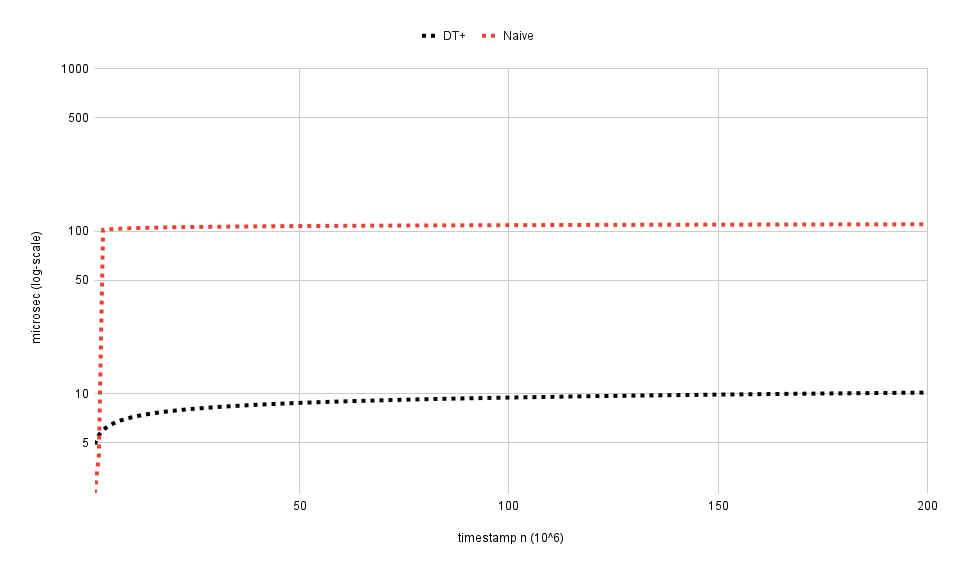
\includegraphics[scale=0.45]{thesis/figures/chart1.1.png}
\caption{Efficiency as a function of time ($m$= 1 million, $\tau$ = 20 million, $k=1$, static queries)}
\end{figure}
\end{center}

As this experiment is designed to purely evaluate the element processing time of each algorithm, we see relatively stable curves once their underlying \textit{structures} have been built. In the case of the naive algorithm, this underlying structure is a simple array containing each query, whereas in the case of the DT+ algorithm, this is the more complicated Endpoint Tree. This explains why the curve for the naive initially starts far below the DT+. However, once the underlying structures are built, we see an observable gap in element processing time which favours our algorithm. As we expect, the cost of element processing for the naive algorithm becomes stable - where the slight uptick in DT+ is due to Distributed Tracking costs, as rounds complete, and new slack values are assigned. Finally, we note that this scaling behaviour matches previous studies on the standard RTS problem \cite{GAN16, DBLP:conf/sigmod/ZhangGBKCZ22}.

We now consider varying values $k$, which represents the number of distinct endpoint functions in our query set. Recall that for \cref{alg:DT+-algorithm}, this will now involve the creation of $k$ DT+ instances to process each endpoint function. In this experiment we know include our bucketing algorithm described in \cref{sec:novel-bucketing-algorithm}. We keep $m$ and $\tau$ as before, though now consider $k = 100,000$. For now, we ignore the approximation factor that comes from using the bucketing algorithm, and instead compare the algorithms based on average processing time. 

\begin{center}
\begin{figure}[h]
\centering
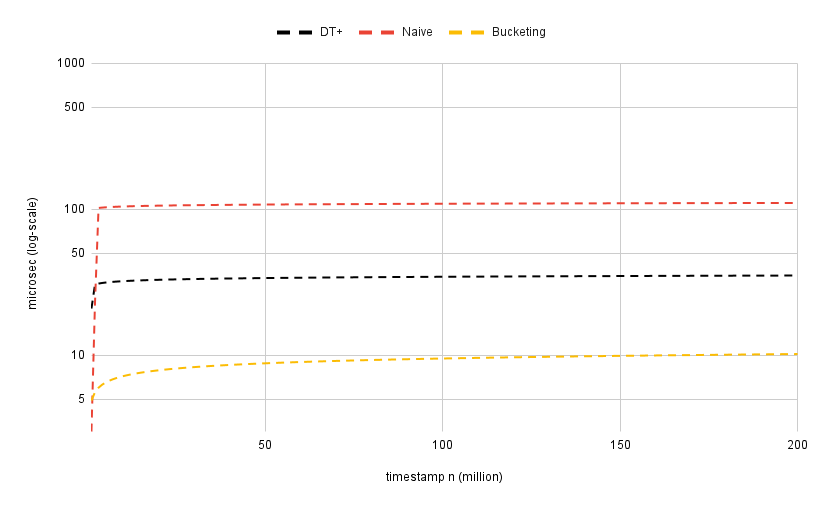
\includegraphics[scale=0.45]{thesis/figures/chart2.1.png}
\caption{Efficiency as a function of time ($m$= 1 million, $\tau$ = 20 million, $k=100,000$ static queries)}
\end{figure}
\end{center}

Here, we see the performance of the DT+ algorithm being much closer to the naive algorithm, which is expected as the algorithm must now perform an additional $k$ loops in each element processing. As predicted by the theory, the Bucketing algorithm remains much more robust - by guaranteeing only a logarithmic factor of loops is performed. 

As before, after the construction of each method, we see the each algorithm stabilise to its average cost of processing. By fixing $m$ and $\tau$, and plotting this stabilised value over $k$, we see that the DT+ algorithm deprecates to performance of the naive approach as $k\to m$. Close inspection shows that the cost of DT+ actually eclipses approach for values of $k$ close to $m$ - the reason lying in the implementation details, as a naive iteration over an array is more efficient than iterating over and tracing through a number of endpoint trees with depths of mostly 1 or 2. Furthermore as we had hoped, we see that the Bucketing algorithm scales much better over $k$.

\begin{center}
\begin{figure}[h]
\centering
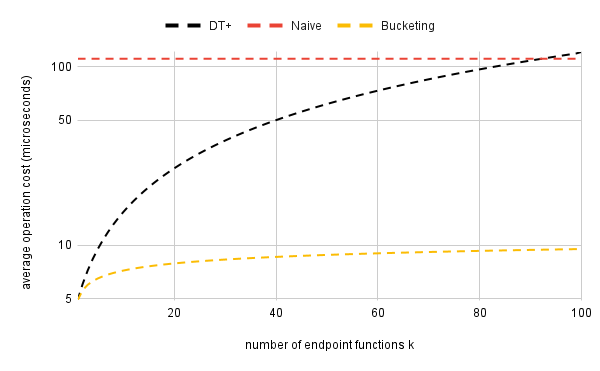
\includegraphics[scale=0.45]{thesis/figures/chart3.1.png}
\caption{Average operation cost over $k$ = number of distinct endpoint functions}
\end{figure}
\end{center}

\newpage
\subsection{Scenario 2: Dynamic Query Insertions}
\label{ssec:experiments-scenario-2}

We now conduct experiments where queries can be inserted and deleted throughout the course of the data stream. 

\textbf{Setup.} Stream elements and queries are generated in the same way as \cref{ssec:experiments-scenario-1}, though the threshold of each query $\tau_q$ is distributed uniformly on $[100, 100,000]$. Across all simulations, the total number of stream elements is fixed at 3 million. Before the stream commences, we register 1 million queries, with other queries added according to a mode of dynamism below: 
\begin{itemize}
    \item \textit{Stochastic Mode}: we fix a parameter $p_{ins}\in(0,1)$ to our simulation, which at each timestamp, an additional query is generated and inserted with probability $p_{ins}$. Similarly, we also supply a parameter $p_{del}\in(0,1)$ which deletes a random live query with probability $p_{del}$. 
    \item \textit{Fixed-load Mode}: As soon as a query is matured or registered, we instantly generate and insert a new one. This ensures that we have a fixed load of live queries over the life of the simulation.
\end{itemize}

\textbf{Results (Stochastic Mode).} First we focus on $p_{ins} = p_{del} = 1/3$, Figure 4.4 shows that the averaged cost per-operation as a function of the number of received elements. The overall trends and relative performance of the algorithms reflect what we have seen so far in the static insertion scenario: 

\begin{center}
\begin{figure}[h]
\centering
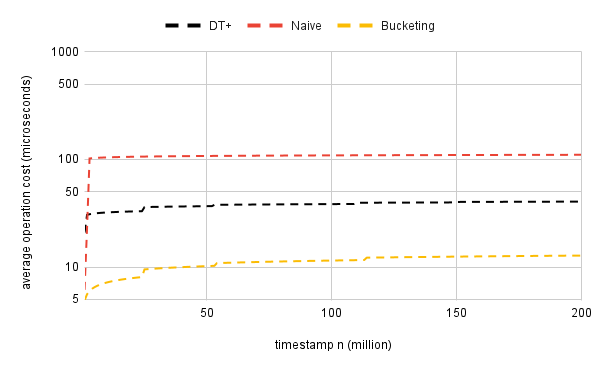
\includegraphics[scale=0.45]{thesis/figures/chart4.1.png}
\caption{Efficiency as a function of time  ($k=100,000$, dynamic queries)}
\end{figure}
\end{center}

It is worth noting that the presence of the occasional bumps in the DT+ and Bucketing chart are the result of logarithmic rebuilding, or global reconstruction taking place as the result of significant query maturation or insertion.

Next, we sought to evaluate how algorithms scale with the rate of insertion. To do so, we adjusted $p_{ins}$ over equally-spaced intervals between 0.1 to 0.5 to and measured the total running time of each algorithm to process the whole stream. As one would be expect, the running time increased linearly in $p_{ins}$.

\begin{center}
\begin{figure}[h]
\centering
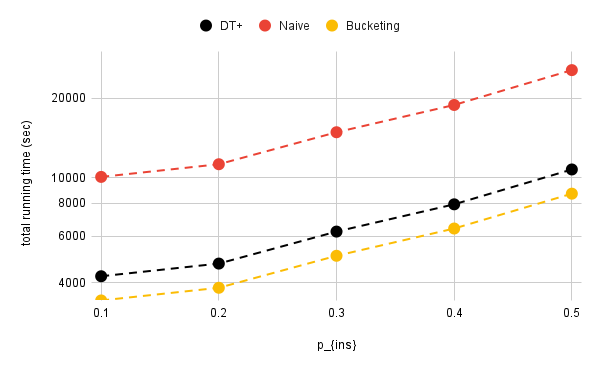
\includegraphics[scale=0.45]{thesis/figures/chart5.1.png}
\caption{Total Stream processing time ($k=10,000$, dynamic queries)}
\end{figure}
\end{center}


\newpage
\subsection{Scenario 3: Performance on Financial Data}
As a final measure of performance, we move from synthetically generated data and instead measure evaluate each algorithm against actual, high frequency trading data. The motivation for this final evaluation is two fold: first, we can gain insight to the performance of our algorithms on actual data streams that are drawn from far more complex distributions than we what have tested so far. Secondly, we can evaluate on DRTS queries with more complex endpoint functions besides the equal step case. 

We choose to set our final experiments in the context of high-frequency trading for both the abundance of quality data sets available, and as a nod to our initial motivation for studying such queries as outlined in \cref{sec:motivation}. We consider high-frequency limit order book data across 5 of the largest and most liquid US technology stocks Amazon, Apple, Google, Intel and Microsoft. All data sets are available and sourced from \href{https://lobsterdata.com/info/DataSamples.php}{LOBSTER} which is used in a number of other studies involving high-frequency financial time series data \cite{RePEc:hum:wpaper:sfb649dp2014-053}